\documentclass[handout,instructornotes]{ximera}
%handout:  for handout version with no solutions or instructor notes
%handout,instructornotes:  for instructor version with just problems and notes, no solutions
%noinstructornotes:  shows only problem and solutions

%% handout
%% space
%% newpage
%% numbers
%% nooutcomes

%I added the commands here so that I would't have to keep looking them up
%\newcommand{\RR}{\mathbb R}
%\renewcommand{\d}{\,d}
%\newcommand{\dd}[2][]{\frac{d #1}{d #2}}
%\renewcommand{\l}{\ell}
%\newcommand{\ddx}{\frac{d}{dx}}
%\everymath{\displaystyle}
%\newcommand{\dfn}{\textbf}
%\newcommand{\eval}[1]{\bigg[ #1 \bigg]}

%\begin{image}
%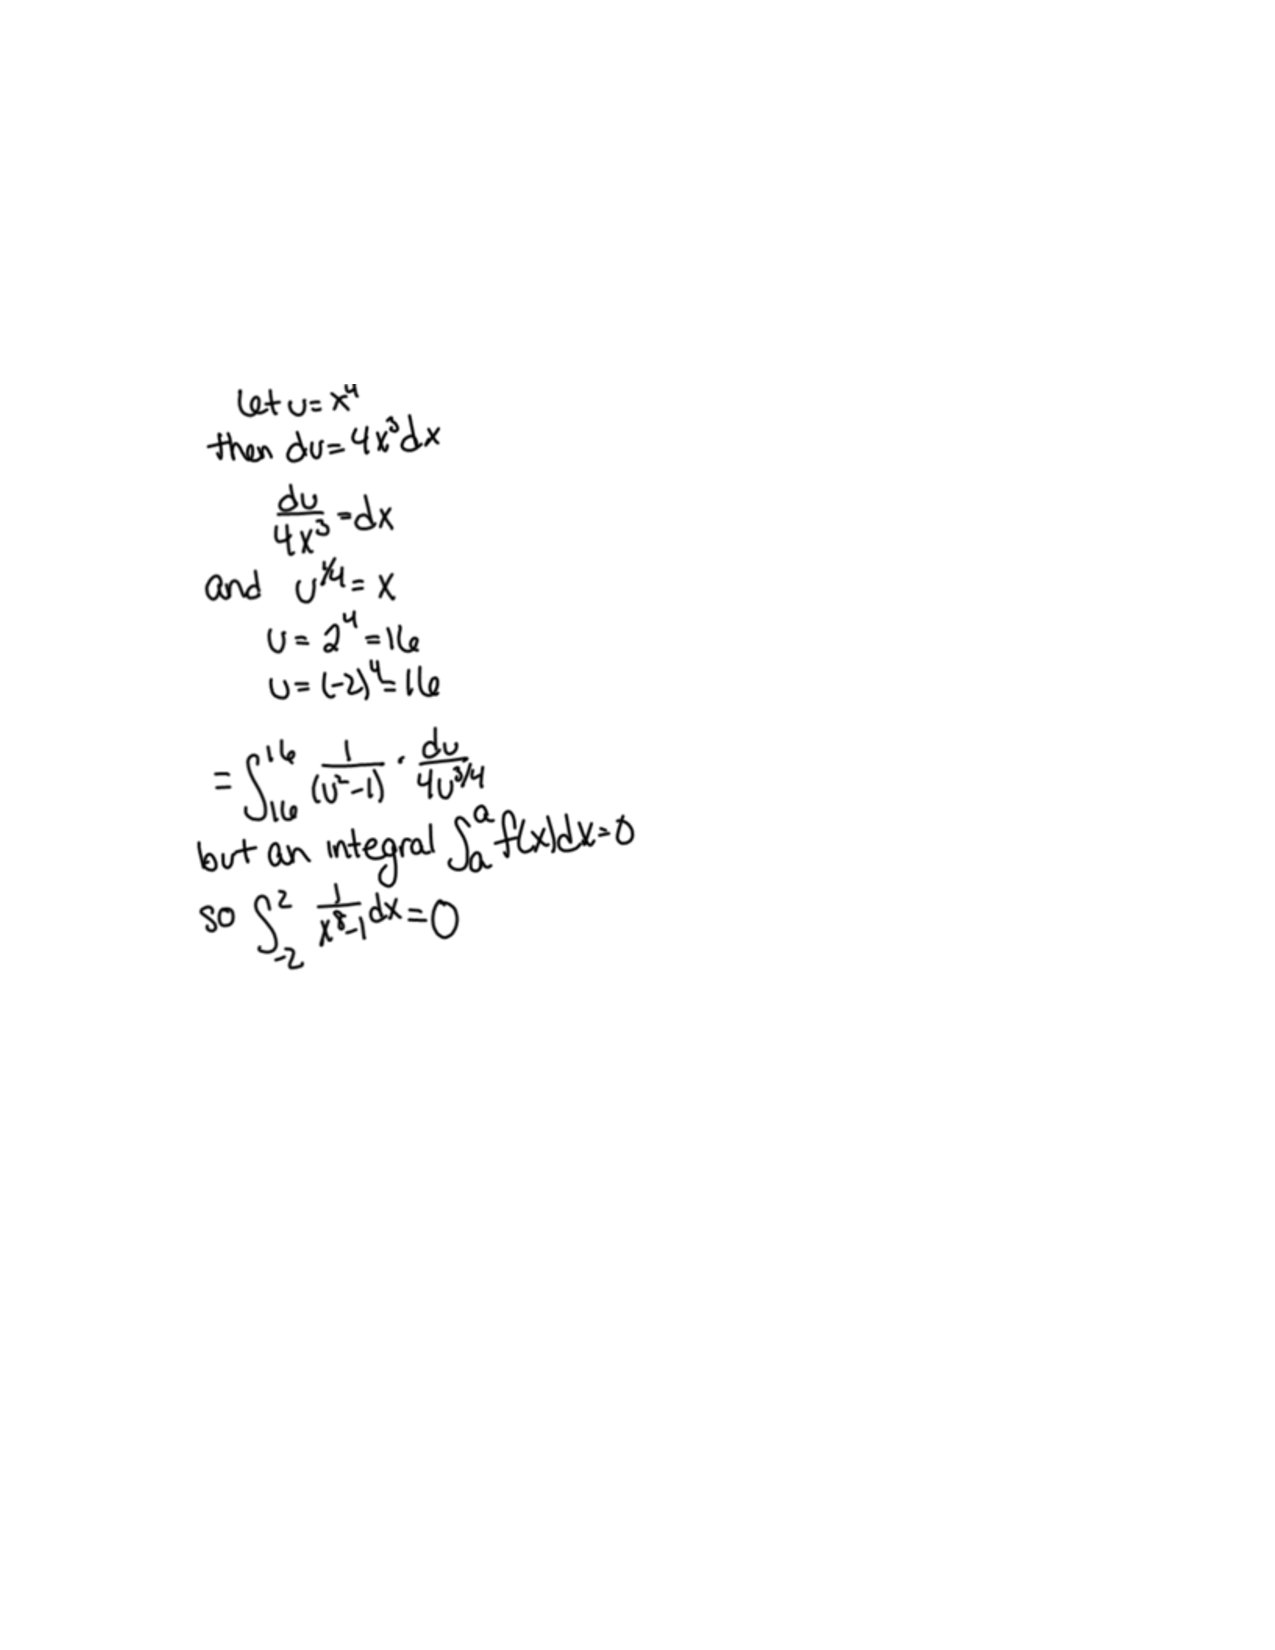
\includegraphics[trim= 170 420 250 180]{Figure1.pdf}
%\end{image}

%add a ``.'' below when used in a specific directory.
\newcommand{\RR}{\mathbb R}
\renewcommand{\d}{\,d}
\newcommand{\dd}[2][]{\frac{d #1}{d #2}}
\renewcommand{\l}{\ell}
\newcommand{\ddx}{\frac{d}{dx}}
\newcommand{\dfn}{\textbf}
\newcommand{\eval}[1]{\bigg[ #1 \bigg]}

\usepackage{multicol}

\renewenvironment{freeResponse}{
\ifhandout\setbox0\vbox\bgroup\else
\begin{trivlist}\item[\hskip \labelsep\bfseries Solution:\hspace{2ex}]
\fi}
{\ifhandout\egroup\else
\end{trivlist}
\fi} %% we can turn off input when making a master document

\title{Recitation \#21: Taylor series - Instructor Notes}  

\begin{document}
\begin{abstract}		\end{abstract}
\maketitle



\section{Warm up:}
Find the Taylor series for:  
	\begin{enumerate}
	\item  $27x^2 - 3x + 17$ about $a=1$.  
	\item  $\sin(2x)$ about $a = \frac{\pi}{8}$.  
	\end{enumerate}
	
	\begin{freeResponse}
	\begin{enumerate}
	\item  
	Let $f(x) = 27x^2-3x+17$.  Then
		\begin{align*}
		&f(1) = 27 - 3 + 17 = 41  \\
		&f'(x) = 54x - 3 	\qquad \Longrightarrow 	\qquad	f'(1) = 54-3=51  \\
		&f''(x) = 54 		\qquad	\Longrightarrow	\qquad f''(1) = 54  \\
		&f^{(3)}(x) = 0 	\qquad	\Longrightarrow	\qquad f^{(3)}(1) = 0  \\
		&\qquad \vdots 	\qquad	\qquad	\qquad \qquad \qquad	\vdots  \\
		&f^{(n)}(x) = 0	\qquad	\Longrightarrow	\qquad	f^{(n)}(1) = 0.
		\end{align*}
	So
		\[
		f(x) = \sum_{k=0}^\infty \frac{f^{(k)}(a)}{k!}(x-a)^k = \boxed{41 + 51(x-1) + \frac{54}{2!}(x-1)^2}
		\]
	Lastly, note that if you multiply this out then you will get back the original polynomial.
	
	
	
	\item Let $f(x) = \sin(2x)$.  Then
		\begin{align*}
		&f \left( \frac{\pi}{8} \right) = \sin \left( \frac{2\pi}{8} \right) = \frac{\sqrt{2}}{2}  \\
		&f'(x) = 2 \cos(2x) 	\qquad \Longrightarrow 	\qquad	f'\left( \frac{\pi}{8} \right) = 2 \cdot \frac{\sqrt{2}}{2} = \sqrt{2}  \\
		&f''(x) = -4 \sin(2x) 		\qquad	\Longrightarrow	\qquad f''\left( \frac{\pi}{8} \right) = -4 \cdot \frac{\sqrt{2}}{2} = -2 \sqrt{2}  \\
		&f^{(3)}(x) = -8 \cos(2x)	\qquad	\Longrightarrow	\qquad f^{(3)}\left( \frac{\pi}{8} \right) = -8 \cdot \frac{\sqrt{2}}{2} = -4 \sqrt{2}  \\
		&f^{(4)}(x) = 16 \cos(2x) \qquad 	\Longrightarrow	\qquad f^{(4)}\left( \frac{\pi}{8} \right) =16 \cdot \frac{\sqrt{2}}{2}  = 8 \sqrt{2}.
		\end{align*}
	Continuing this pattern, we see that
		\[
		f^{(k)} \left( \frac{\pi}{8} \right) = (-1)^{\left\lceil \frac{k}{2} \right\rceil } 2^{k-1} \sqrt{2}
		\]
	where $\left\lceil \frac{k}{2} \right\rceil$ denotes the smallest integer greater than $\frac{k}{2}$.  
	So, for example, $\left\lceil \frac{1}{2} \right\rceil = 1$, $\left\lceil \frac{2}{2} \right\rceil = 1$, $\left\lceil \frac{3}{2} \right\rceil = 2$, and so on.  
	
	So from here we have that the Taylor series for $f(x)$ is
		\[
		\boxed{\sum_{k=0}^\infty \frac{(-1)^{\left\lceil \frac{k}{2} \right\rceil } 2^{k-1} \sqrt{2}}{k!} \left( x - \frac{\pi}{8} \right)^k}
		\]
	
	\end{enumerate}
	\end{freeResponse}
	
\begin{instructorNotes}
Here, they need to compute the Taylor series by computing derivatives and recognizing patterns.  

Part (a) is an opportunity to show the students that a polynomial is already a Maclaurin series.  
Use derivatives to figure out the Taylor series about $a=1$, and then show them that the answer simplifies back to the original problem.  

Part (b) is a continuation from the previous recitation where they already found the approximating polynomial.  
The students may have a problem finding the pattern in the derivatives (especially with the alternating part).
\end{instructorNotes}







\section{Group work:}



%problem 1
\begin{problem}
Find a power series (and interval of convergence) for each of the following functions
	\begin{multicols}{2}
	\begin{enumerate}
	\item  $f(x) = x^3 \sin(x^5)$
	\item  $f(x) = \frac{1}{(1+x)^4}$
	\item  $f(x) = \frac{1}{(3-5x^2)^4}$
	\item  $f(x) = \sin^{-1}(x^5)$
	\end{enumerate}
	\end{multicols}
	
	\begin{freeResponse}
	\begin{enumerate}
	\item  We already know that 
		\[
		\sin x = \sum_{k=0}^\infty \frac{(-1)^k x^{2k+1}}{(2k+1)!}
		\]
	with interval of convergence $( - \infty, \infty)$.  
	So we use this to compute
		\begin{align*}
		x^3 \sin(x^5) &= x^3 \sum_{k=0}^\infty \frac{(-1)^k (x^5)^{2k+1}}{(2k+1)!}  \\
		&= x^3 \sum_{k=0}^\infty \frac{(-1)^k x^{10k+5}}{(2k+1)!}  \\
		&= \boxed{\sum_{k=0}^\infty \frac{(-1)^k x^{10k+8}}{(2k+1)!}}
		\end{align*}
	with interval of convergence $( - \infty, \infty)$.  
	
	
	
	\item  Recall that the {\it Binomial Series} has the power series representation
		\[
		(1+x)^p = \sum_{k=0}^\infty {{p}\choose{k}} x^k
		\]
	with interval of convergence $(-1,1)$, and where
		\[
		{{p}\choose{k}} = \frac{p(p-1)(p-2) \hdots (p-k+1)}{k!}.
		\]
	So
		\begin{align*}
		f(x) &= (1+x)^{-4}  \\
		&= \boxed{\sum_{k=0}^\infty {{-4}\choose{k}} x^k}
		\end{align*}
	with interval of convergence $(-1,1)$.  
	
	
	
	\item  Just as in part (b), we have that
		\begin{align*}
		f(x) &= \frac{1}{(3-5x^2)^4}  \\
		&= (3-5x^2)^{-4}  \\
		&= 3^{-4} \left( 1 - \frac{5}{3}x^2 \right)^{-4}  \\
		&= 3^{-4} \sum_{k=0}^\infty {{-4}\choose{k}} \left( - \frac{5}{3} x^2 \right)^k   \\
		&= \boxed{\sum_{k=0}^\infty (-1)^k {{-4}\choose{k}} \frac{5^k x^{2k}}{3^{k+4}}}.
		\end{align*}
	To find the interval of convergence, we know that we must have
		\[
		\biggr| - \frac{5}{3} x^2 \biggr| < 1.
		\]
	So we solve
		\begin{align*}
		&\biggr| - \frac{5}{3} x^2 \biggr| < 1  \\
		\Longleftrightarrow	\qquad	&\frac{5}{3} x^2 < 1  \\
		\Longleftrightarrow	\qquad	&x^2 < \frac{3}{5}  \\
		\Longleftrightarrow	\qquad	&- \sqrt{\frac{3}{5}} < x < \sqrt{\frac{3}{5}}.
		\end{align*}
	Thus, the interval of convergence is $\boxed{ \left( - \sqrt{\frac{3}{5}}, \sqrt{\frac{3}{5}} \right) }$.
	
	
	
	\item  Let us first consider $g(x) = \arcsin(x)$.  
	Then 
		\begin{align*}
		g'(x) &= \frac{1}{\sqrt{1-x^2}}   \\
		&= (1-x^2)^{- \frac{1}{2}}  \\
		&= \sum_{k=0}^\infty {{- \frac{1}{2}}\choose{k}} (-x^2)^k  \\
		&= \sum_{k=0}^\infty (-1)^k {{- \frac{1}{2}}\choose{k}} x^{2k}
		\end{align*}
	To find the interval of convergence, we need
		\[
		|-x^2| < 1 	\qquad \Longleftrightarrow \qquad x^2 < 1 \qquad \Longleftrightarrow \qquad -1 < x < 1.
		\] 
	So the interval of convergence for $g'(x)$ is $(-1,1)$.  
	
	Now,
		\begin{align*}
		g(x) &= \int g'(x) \d x  \\
		&=  \sum_{k=0}^\infty (-1)^k {{- \frac{1}{2}}\choose{k}} \frac{x^{2k+1}}{2k+1} + C  
		\end{align*}
	which also has IOC $(-1,1)$, since integrating will not change the IOC of a binomial series.  
	To find $C$, we just evaluate at $x=0$:
		\[
		0 = \arcsin(0) = g(0) = \sum_{k=0}^\infty (-1)^k {{- \frac{1}{2}}\choose{k}} \frac{0^{2k+1}}{2k+1} + C = 0 + C
		\]
	and so $C=0$.  Therefore, we have that
		\[
		g(x) = \sum_{k=0}^\infty (-1)^k {{- \frac{1}{2}}\choose{k}} \frac{x^{2k+1}}{2k+1}
		\]
	on $(-1,1)$.  
	
	Finally, $f(x) = \arcsin(x^5) = g(x^5)$.  So
		\begin{align*}
		f(x) &= \sum_{k=0}^\infty (-1)^k {{- \frac{1}{2}}\choose{k}} \frac{(x^5)^{2k+1}}{2k+1}  \\
		&= \boxed{\sum_{k=0}^\infty (-1)^k {{- \frac{1}{2}}\choose{k}} \frac{x^{10k+5}}{2k+1}}
		\end{align*}
	with interval of convergence $(-1,1)$ (since $|x^5| < 1$ if and only if $|x| < 1$).  
		  
	
	\end{enumerate}
	\end{freeResponse}
	
\end{problem}

\begin{instructorNotes}
Students should use the known Maclaurin series in various ways.  
You might want to give the hint in part (d) that $\ddx \sin^{-1}(x) = \frac{1}{\sqrt{1-x^2}}$.  
\end{instructorNotes}







%problem 2
\begin{problem}
Find a function (closed expression) for the following series and the interval on which the function and the series are equal.
	\[
	x + x^4 + \frac{1}{2} x^7 + \frac{1}{6} x^{10} + \frac{1}{24} x^{13} + \hdots
	\]
	\begin{freeResponse}
		\begin{align*}
		x + x^4 + \frac{1}{2} x^7 + \frac{1}{6} x^{10} + \frac{1}{24} x^{13} + \hdots
		&= x + x^4 + \frac{1}{2!} x^7 + \frac{1}{3!} x^{10} + \frac{1}{4!} x^{13} + \hdots  \\
		&= \sum_{k=0}^\infty \frac{1}{k!}x^{3k + 1}  \\
		&= x \sum_{k=0}^\infty \frac{x^{3k}}{k!}  \\
		&= x \sum_{k=0}^\infty \frac{(x^3)^k}{k!}  \\
		&= \boxed{xe^{x^3}}
		\end{align*}
	which has interval of convergence $(- \infty, \infty)$.  
	\end{freeResponse}
		
\end{problem}

\begin{instructorNotes}
The students need to rewrite $f(x)$ in summation notation (factoring out an $x$) and seeing the series for $xe^{x^3}$.  
\end{instructorNotes}







%problem 3
\begin{problem}
Compute the sum of the following series ({\it Hint:  You should use Taylor series.})
	\begin{enumerate}
	\item  $1 - \ln 2 + \frac{(\ln 2)^2}{2!} - \frac{(\ln 2)^3}{3!} + \hdots$
	\item  $3 + \frac{9}{2!} + \frac{27}{3!} + \frac{81}{4!} + \hdots$
	\end{enumerate}
	
	\begin{freeResponse}
	\begin{enumerate}
	\item  
		\begin{align*}
		1 - \ln 2 + \frac{(\ln 2)^2}{2!} - \frac{(\ln 2)^3}{3!} + \hdots
		&= \sum_{k=0}^\infty \frac{(- \ln 2)^k}{k!}  \\
		&= e^{- \ln 2}  = e^{\ln 2^{-1}}  \\
		&= 2^{-1} = \boxed{\frac{1}{2}}.
		\end{align*}
	
	
	
	\item  
		\begin{align*}
		3 + \frac{9}{2!} + \frac{27}{3!} + \frac{81}{4!} + \hdots
		&= \sum_{k=1}^\infty \frac{3^k}{k!}  \\
		&= \sum_{k=0}^\infty \frac{3^k}{k!} - \frac{3^0}{0!}  \\
		&= \boxed{e^3 - 1}.
		\end{align*}
	
	\end{enumerate}
	\end{freeResponse}

\end{problem}

\begin{instructorNotes}
The goal here is for students to realize that Taylor series gives them a tool for finding the exact sum of a series.
\end{instructorNotes}
















	
	
	
	
	
	
	
	
	

	










								
				
				
	














\end{document} 


















